% PrepTalk -- technical report, HackApertus 2026, Track 2A (FHGR). Build: make report (pdflatex, twice).
\documentclass[10pt,a4paper]{article}

% ---------------------------------------------------------------- links and historical consistency numbers
\newcommand{\repository}{\href{https://github.com/ghwiegand/PrepTalk}{github.com/ghwiegand/PrepTalk}}
\newcommand{\videolink}{} % Add the demo URL when available; the empty field is hidden below.
\newcommand{\spread}{Per scenario run, Opus ranges from 0 to 100\,\% (mean 64, SD 26), Gemini Pro from 40 to 100\,\% (mean 74, SD 20).}
\newcommand{\callslang}{de 3.04, fr 3.07, it 3.07}


% ---------------------------------------------------------------- packages
\usepackage[T1]{fontenc}
\usepackage[utf8]{inputenc}
\usepackage[english]{babel}
\usepackage{newtxtext,newtxmath}
\usepackage[scaled=0.95]{sourcesanspro}
\renewcommand{\familydefault}{\rmdefault}
\ifPDFTeX
  \usepackage[varqu]{inconsolata}
\else
  \setmonofont{lmmono10-regular.otf}[Scale=MatchLowercase]
\fi
\usepackage[a4paper,margin=2.1cm,top=2.3cm,bottom=2.4cm]{geometry}
\usepackage{microtype}
\usepackage[table]{xcolor}
\usepackage{graphicx}
\usepackage{booktabs,tabularx,array,multirow}
\usepackage{enumitem}
\usepackage{titlesec}
\usepackage{fancyhdr}
\usepackage[font=small,labelfont={bf,sf},labelsep=period]{caption}
\usepackage[most]{tcolorbox}
\usepackage{tikz}
\usetikzlibrary{arrows.meta,positioning,shapes.geometric,fit,backgrounds}
\usepackage[hidelinks]{hyperref}


\definecolor{navy}{HTML}{1B2440}
\definecolor{rust}{HTML}{A8441F}
\definecolor{steel}{HTML}{2C5D8A}
\definecolor{paper}{HTML}{F5F3EE}
\definecolor{ink}{HTML}{3A3F4B}
\definecolor{okgreen}{HTML}{2E7D4F}

\graphicspath{{../}{./}}
\setlength{\parindent}{0pt}
\setlength{\parskip}{4.5pt}
\setlength{\emergencystretch}{2em}
\setlist{nosep,leftmargin=1.2em,itemsep=1.5pt,topsep=2pt}
\renewcommand{\arraystretch}{1.18}

\titleformat{\section}{\sffamily\bfseries\large\color{navy}}{\thesection}{0.6em}{}
\titleformat{\subsection}{\sffamily\bfseries\normalsize\color{navy}}{\thesubsection}{0.5em}{}
\titleformat{\paragraph}[runin]{\sffamily\bfseries\small\color{rust}}{}{0pt}{}[.]
\titlespacing*{\section}{0pt}{12pt}{4pt}
\titlespacing*{\subsection}{0pt}{8pt}{3pt}
\titlespacing*{\paragraph}{0pt}{4pt}{0.6em}

\pagestyle{fancy}
\fancyhf{}
\renewcommand{\headrulewidth}{0pt}
\fancyfoot[L]{\sffamily\scriptsize\color{ink}HackApertus 2026 \textperiodcentered{} Track 2A \textperiodcentered{} FHGR \textperiodcentered{} PrepTalk, Team NLP-Lab}
\fancyfoot[R]{\sffamily\scriptsize\color{ink}\thepage}

% criterion tags: which judging criterion a section serves
\newcommand{\crit}[2]{\tcbox[on line,colback=#1,colframe=#1,coltext=white,boxsep=0pt,left=3pt,right=3pt,top=1.5pt,bottom=1.5pt,arc=2pt,fontupper=\sffamily\bfseries\scriptsize]{#2}}
\newcommand{\perf}{\crit{steel}{Performance 50\,\%}}
\newcommand{\cons}{\crit{navy}{Consistency 25\,\%}}
\newcommand{\inno}{\crit{rust}{Innovation 25\,\%}}
\newcommand{\gate}{\crit{okgreen}{Required gate}}

\newtcolorbox{keybox}[1][]{enhanced,colback=paper,colframe=paper,arc=3pt,boxrule=0pt,left=8pt,right=8pt,top=6pt,bottom=6pt,
  borderline west={2.5pt}{0pt}{rust},#1}
\newtcolorbox{dialog}[1]{enhanced,colback=white,colframe=navy!25,arc=2pt,boxrule=0.5pt,left=6pt,right=6pt,top=4pt,bottom=4pt,
  title={\sffamily\bfseries\scriptsize #1},coltitle=navy,colbacktitle=navy!8,attach boxed title to top left={xshift=6pt,yshift=-2pt},
  boxed title style={boxrule=0pt,arc=2pt},fontupper=\small}
\newcommand{\coach}[1]{\par\noindent\hangindent=4.2em\hangafter=1\makebox[4.2em][l]{\sffamily\bfseries\scriptsize\color{steel}COACH}#1}
\newcommand{\cand}[1]{\par\noindent\hangindent=4.2em\hangafter=1\makebox[4.2em][l]{\sffamily\bfseries\scriptsize\color{ink}APPLICANT}\textit{#1}}
\newcommand{\note}[1]{\par\noindent\hspace*{4.2em}{\sffamily\scriptsize\color{rust}$\blacktriangleright$ #1}}

\hypersetup{pdftitle={PrepTalk: technical report},pdfauthor={Team NLP-Lab}}

\begin{document}

% ================================================================ title
\begin{tcolorbox}[enhanced,colback=navy,colframe=navy,arc=0pt,boxrule=0pt,left=14pt,right=14pt,top=12pt,bottom=12pt,
  coltext=white,width=\textwidth]
{\sffamily\bfseries\footnotesize\color{rust!60!white}HACKAPERTUS 2026 \textperiodcentered{} TRACK 2A \textperiodcentered{} FHGR: AI-POWERED JOB INTERVIEW COACH}\\[6pt]
{\fontsize{24}{28}\selectfont\bfseries PrepTalk}\\[3pt]
{\large An interview coach in which Apertus talks and judges, and a rule engine decides}\\[8pt]
{\sffamily\small Team NLP-Lab \textperiodcentered{} Götz-Henrik Wiegand (PhD student, University of St.\,Gallen) \textperiodcentered{} Online\\[2pt]
Code: \repository{} \textperiodcentered{}
\ifdefempty{\videolink}{Demo video: accompanying submission}{\href{\videolink}{Demo video}}}
\end{tcolorbox}

\vspace{2pt}
% ================================================================ page 1: purpose and requirements
\section*{Summary}
PrepTalk helps 14--16-year-olds practise a Swiss apprenticeship interview in German, French or Italian.
It asks occupation-specific questions, follows up on vague answers, answers the candidate's questions as the
company, and then switches to coaching with evidence from the conversation and a concrete next step.
Swiss German answers are accepted; the coach replies in Standard German.

Apertus~1.5~8B phrases reactions and follow-ups, judges answers and writes feedback contents.
\textbf{FrameX controls the interview}: explicit rules determine question order, reasks, follow-ups and the
transition to feedback. Deterministic checks constrain model output, with fixed fallbacks for failed calls.
This separates fluent wording from the decisions that make an interview useful and repeatable.

\begin{keybox}
\textbf{Reported evaluation.} The original evaluation used synthetic applicants, two independent model judges
and a separate comparison with FHGR reference feedback. The final coach met the project's regression checks
in all 28 scenario interviews and averaged about \textbf{3.1 model calls per candidate answer}.
Against FHGR's reference feedback, levels were within one step in \textbf{100\,\% of 141 assessed criteria};
\textbf{87\,\%} of evidence excerpts were verbatim. These are development results, not the official benchmark
or a study with real teenagers.
\end{keybox}

\subsection*{How PrepTalk addresses the challenge}
\begin{center}\small
\begin{tabularx}{\textwidth}{@{}>{\raggedright\arraybackslash}p{3.6cm}>{\raggedright\arraybackslash}X@{}}
\toprule
\sffamily\bfseries Requirement & \sffamily\bfseries Implementation and evidence \\
\midrule
Apertus 1.5 8B & \texttt{swiss-ai/Apertus-v1.5-8B}, inference only, temperature 0; vLLM serving. \\
Local deployment, $<$\,32\,GB VRAM & Docker GPU profile; bf16 weights need about 16\,GB, plus serving overhead. Evaluation used one NVIDIA L4. \\
$<$\,5 calls per answer & Guard, reaction and judgement, with extra calls for company answers and feedback; about 3.1 on average. \\
Adaptive interview & Situation-specific plans, profile-conditional questions, one reask and targeted follow-ups. \\
Constructive feedback & 11 criteria, four levels, evidence, up to two improvement points and one practice task. \\
Multilingual and voice-ready & de/fr/it; dialect-aware checks; spoken feedback rendering and an experimental local macOS voice client. \\
Reproducible deliverables & Source, Docker stack, README, visual architecture and evaluation scripts. \\
\bottomrule
\end{tabularx}
\end{center}

\subsection*{Reading the evidence}
The report follows the judging dimensions: \perf{} (Section~\ref{sec:perf}),
\cons{} (Section~\ref{sec:cons}) and \inno{} (Section~\ref{sec:inno}).
The rules comparison, group breakdown and reference-feedback study are identified separately.
Technical constraints and model use are described next; limitations, reproduction commands and disclosure
close the report.

% ================================================================ page 2: architecture and model
\clearpage
\section{Architecture and use of Apertus}\label{sec:arch}\label{sec:apertus}
\begin{center}
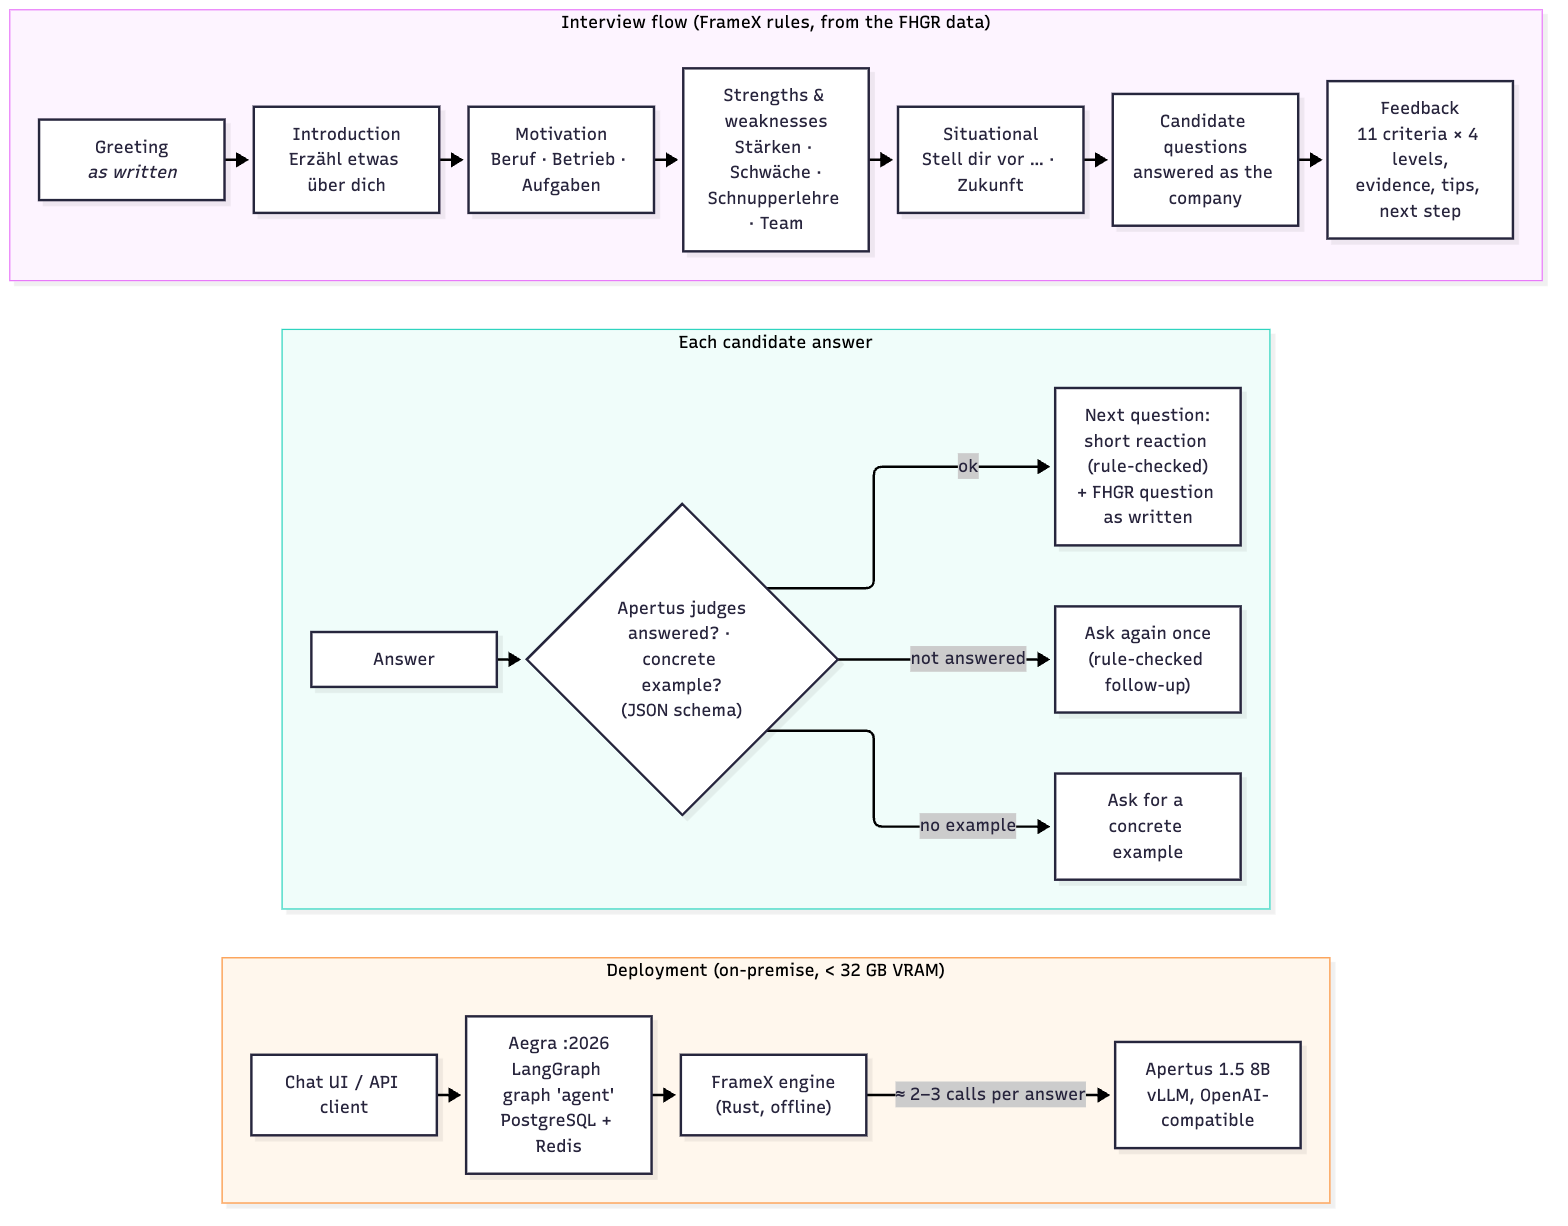
\includegraphics[width=0.94\textwidth]{architecture.png}
\captionof{figure}{Interview flow, turn processing and deployment. The generated FrameX program selects the
next action; Apertus supplies judgements and wording through an OpenAI-compatible endpoint.}
\label{fig:arch}
\end{center}

\paragraph{Interview plan and state}
FHGR's question bank supplies six stages: introduction, motivation, strengths and weaknesses,
situational questions, candidate questions and feedback. Six situations have tailored plans of usually
8--12 main questions (phone calls: three), including occupation-specific and profile-conditional questions.
Each turn replays recorded tool results without model calls, consumes the pending answer and continues
until input is needed. JSON state lives in LangGraph checkpoints; shared FrameX globals require
serialized turns within a process.

\paragraph{Model roles and fallbacks}
Apertus reacts, judges, answers as the company and fills feedback contents. A normal answer costs a guard
call, reaction and judgement with a follow-up check; pattern-matched guards avoid a call.
\texttt{json\_schema} falls back to \texttt{json\_object} for rejected schemas. Failed calls use neutral
wording, fixed questions or rule-based judgements. Company answers are checked against posting facts;
Swiss training terms use a glossary.

\paragraph{Coaching and voice}
Distress pauses the interview with support and referral; manipulation redirects to the pending question.
A feedback request ends early. Checked feedback (Section~\ref{sec:feedback}) can be rendered for speech
with \texttt{voice: true}. An experimental macOS client adds local Whisper base transcription via
whisper.cpp and system-voice playback; it was not part of the reported evaluation.

\paragraph{User interface and demo}
The terminal interface supports scenario, apprenticeship posting and language selection, followed by a
guided interview with progress indicators. The
\ifdefempty{\videolink}{accompanying demo video, submitted with this report,}{\href{\videolink}{accompanying demo video}}
shows adaptive follow-ups, support for distress, resistance to manipulation, feedback with conversation
evidence and an exported decision trace.

\paragraph{Serving and data}
\texttt{LLM\_BASE\_URL} selects the OpenAI-compatible Apertus endpoint. The GPU profile uses Swiss AI's
vLLM image, bf16 and a 16,384-token context. FHGR data is fetched at a pinned revision rather than
redistributed. Evaluation candidates and companies are fictional; interactive state is stored in checkpoints.

% ================================================================ page 3: supplied rules comparison
\clearpage
\section{Evaluation: performance}\label{sec:perf}
\perf{}\quad
The evaluation separates interview quality from hard regression checks. Independent judges,
Claude Opus~5.5 and Gemini Pro, assess scenario criteria and five aspects: realism, adaptivity,
feedback quality, age-appropriateness and language consistency. Hard checks count failures directly,
including aborted interviews, wrong-language reactions, third-person feedback and guard-handled text
quoted as evidence. All live coach calls, including retries, count toward the call budget.

\begin{center}\small
\captionof{table}{Rules comparison (28 interviews per configuration). Criteria scores without rules are
pooled; with rules, development / new-scenario scores are shown separately.}
\label{tab:main}
\begin{tabularx}{\textwidth}{@{}>{\raggedright\arraybackslash}X>{\raggedright\arraybackslash}p{3.0cm}>{\raggedright\arraybackslash}p{5.0cm}@{}}
\toprule
\sffamily\bfseries Measure & \sffamily\bfseries Without rules & \sffamily\bfseries With rules \\
\midrule
Interviews passing all hard checks & 3 of 28 & 28 of 28 \\
Scenario criteria met (Opus) & 42\,\% & 67\,\% / 54\,\% \\
Scenario criteria met (Gemini) & 45\,\% & 75\,\% / 67\,\% \\
Model calls per candidate answer & 2.06 & 3.07 \\
\bottomrule
\end{tabularx}
\end{center}

\begin{center}
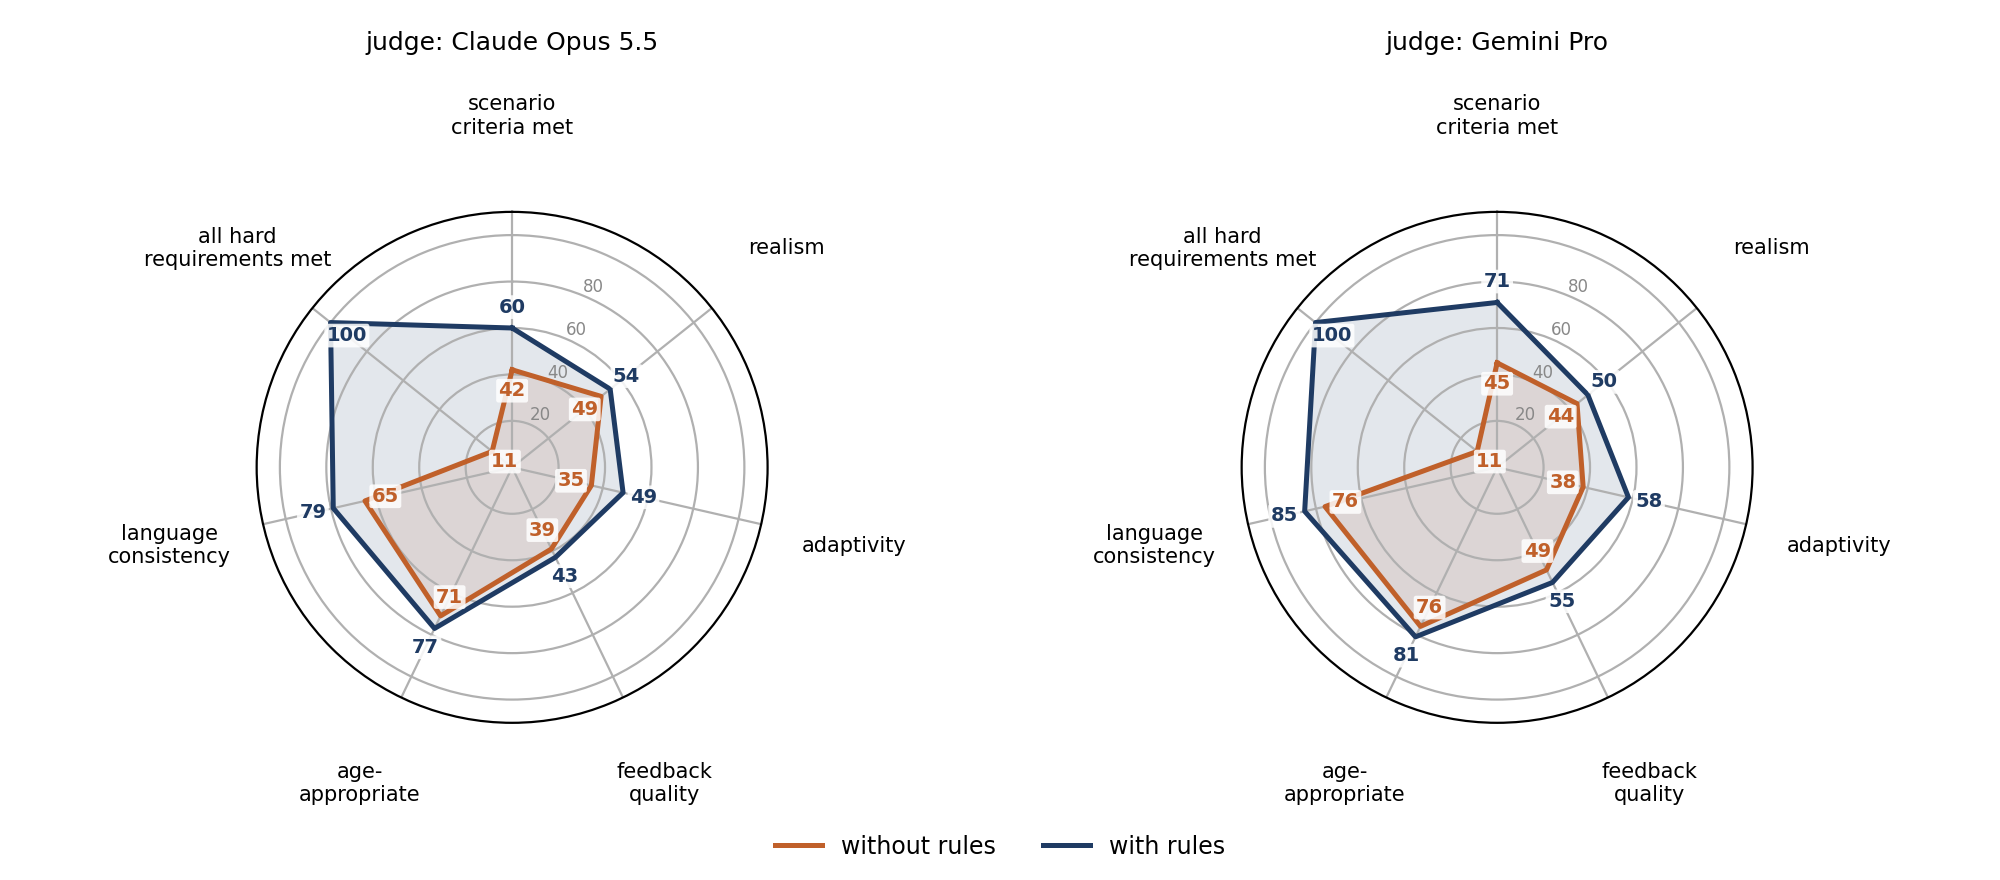
\includegraphics[width=\textwidth]{rules_spider.png}
\captionof{figure}{Both colours represent the Apertus~1.5~8B coach: orange shows Apertus~1.5~8B
without rules; blue shows Apertus~1.5~8B with rules. Claude Opus~5.5 (left) and Gemini Pro (right)
were used only as independent judges to rate the coach's responses on the displayed quality criteria;
they did not generate the coach's responses. The hard-check pass rate is measured by regression checks.
Scenario criteria met and hard-check pass rates are percentages; aspect ratings use a 0--100 display
scale. Read each axis individually.}
\label{fig:results}
\end{center}

\paragraph{Largest gain: reliable execution}
Only three of 28 interviews pass all hard checks without rules (11\,\%, rounded); all pass with rules.
The average call count remains below five despite the added checks. Pooled scenario success rises from
42 to 60\,\% under Opus and from 45 to 71\,\% under Gemini, as shown in Figure~\ref{fig:results}.
Development and new-scenario results are reported separately in Table~\ref{tab:main}; the lower new-scenario
scores leave a generalisation gap.

\paragraph{Quality gains are uneven}
Both judges rate the rule-based version higher on every plotted aspect. The largest visual change is in
hard-check compliance; adaptivity and feedback quality remain weaker than language consistency and
age-appropriateness. Deterministic checks address recurring failure modes, while a follow-up's relevance
and the interpretation of a difficult answer still depend on Apertus.

\paragraph{Reading across experiments}
This rules comparison is reported separately from the earlier per-group consistency breakdown
(Section~\ref{sec:cons}), the FHGR reference-feedback study and the evidence-driven pilot
(Section~\ref{sec:feedback}). The group results below have not been recomputed from this comparison's
aggregate scores; they describe the original evaluation runs.

% ================================================================ page 4: consistency
\clearpage
\section{Evaluation: consistency}\label{sec:cons}
\cons{}\quad
The same flow templates, output checks and fallbacks apply across languages and profiles.
The breakdown below describes the original 28 scenario runs, pooling development and held-out scenarios.
It measures scenario criteria met, not a claim of equal performance across all users.

\begin{center}
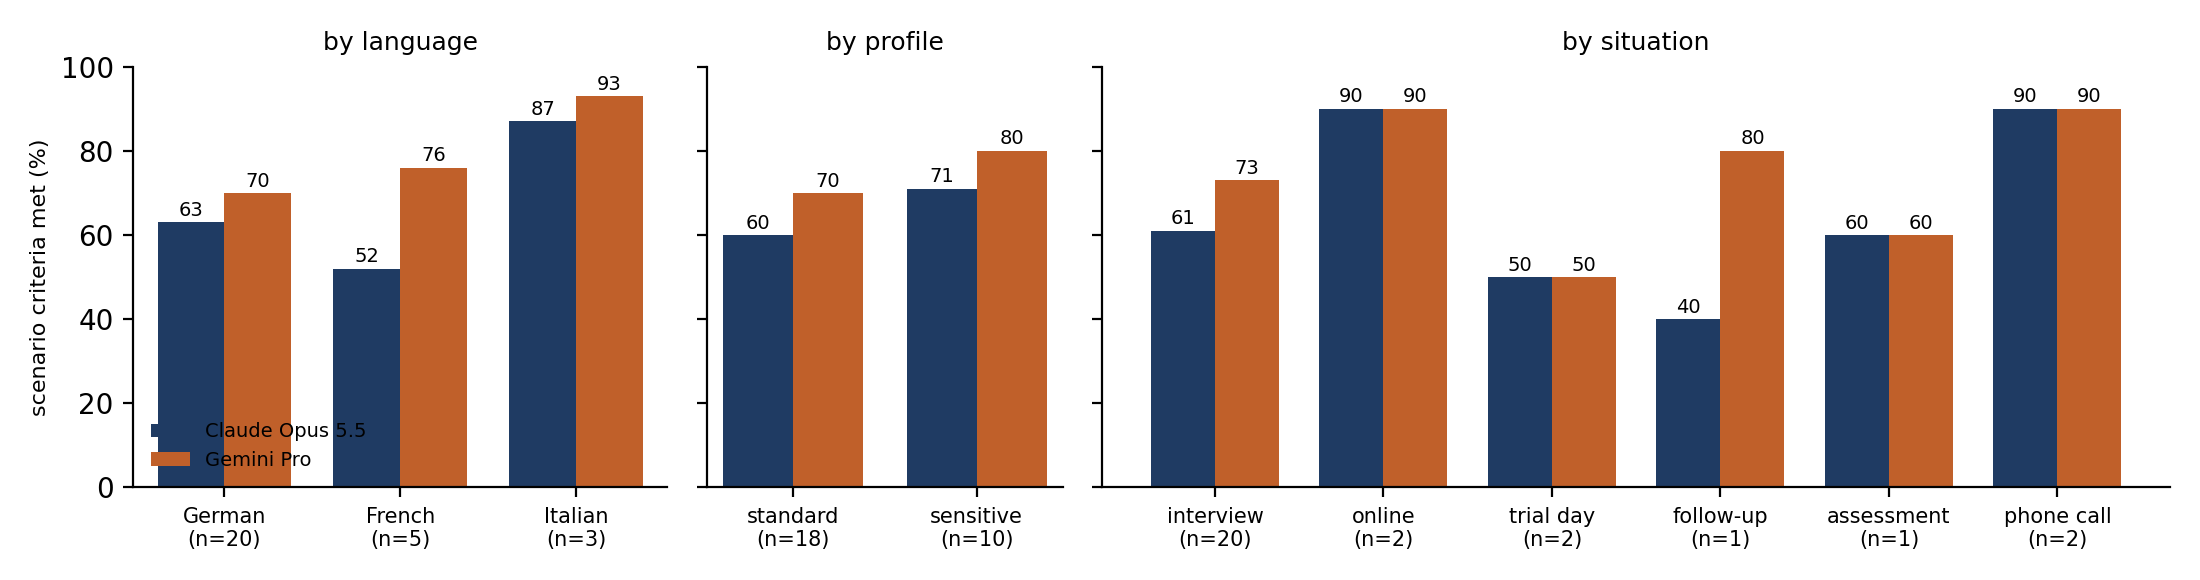
\includegraphics[width=\textwidth]{consistency.png}
\captionof{figure}{Original evaluation by language, profile and situation; $n$ denotes scenario runs.
Sensitive profiles include dyslexia, second-language speakers, interrupted schooling or apprenticeships,
emotional moments, gender-atypical choices, strong self-doubt and dialect speakers.}
\label{fig:cons}
\end{center}

\begin{center}\small
\captionof{table}{Original consistency breakdown: percentage of scenario criteria met, by judge.
Groups are columns; parenthesized counts give the number of scenario runs.}
\label{tab:cons}
\setlength{\tabcolsep}{3pt}
\begin{tabularx}{\textwidth}{@{}l*{10}{>{\centering\arraybackslash}X}@{}}
\toprule
& \multicolumn{3}{c}{\sffamily\bfseries Language}
& \multicolumn{2}{c}{\sffamily\bfseries Profile}
& \multicolumn{2}{c}{\sffamily\bfseries Dialect}
& \multicolumn{3}{c}{\sffamily\bfseries Difficulty} \\
\cmidrule(lr){2-4}\cmidrule(lr){5-6}\cmidrule(lr){7-8}\cmidrule(l){9-11}
\sffamily\bfseries Judge
& \shortstack{German\\(20)} & \shortstack{French\\(5)} & \shortstack{Italian\\(3)}
& \shortstack{Sensitive\\(10)} & \shortstack{Standard\\(18)}
& \shortstack{Dialect\\speaker\\(19)} & \shortstack{Standard\\language\\(9)}
& \shortstack{Easy\\(5)} & \shortstack{Hard\\(5)} & \shortstack{Medium\\(18)} \\
\midrule
Opus & 63\,\% & 52\,\% & 87\,\% & 71\,\% & 60\,\% & 64\,\% & 64\,\% & 76\,\% & 65\,\% & 60\,\% \\
Gemini & 70\,\% & 76\,\% & 93\,\% & 80\,\% & 70\,\% & 71\,\% & 80\,\% & 80\,\% & 81\,\% & 70\,\% \\
\bottomrule
\end{tabularx}

\medskip
\begin{tabularx}{\textwidth}{@{}l*{6}{>{\centering\arraybackslash}X}@{}}
\toprule
& \multicolumn{6}{c}{\sffamily\bfseries Situation} \\
\cmidrule(l){2-7}
\sffamily\bfseries Judge
& \shortstack{Assessment\\(1)} & \shortstack{Follow-up\\(1)} & \shortstack{Interview\\(20)}
& \shortstack{Online\\(2)} & \shortstack{Phone call\\(2)} & \shortstack{Trial day\\(2)} \\
\midrule
Opus & 60\,\% & 40\,\% & 61\,\% & 90\,\% & 90\,\% & 50\,\% \\
Gemini & 60\,\% & 80\,\% & 73\,\% & 90\,\% & 90\,\% & 50\,\% \\
\bottomrule
\end{tabularx}
\end{center}

\paragraph{What is stable, and what varies}
The original regression checks passed in all 28 interviews; calls per answer were similar across languages
(\callslang). Sensitive profiles scored above standard profiles in this sample, while French scored lower
than German or Italian under Opus. These small, differently composed groups do not establish fairness or
a language effect. \spread{} Several situation groups contain only one or two scenarios.

\paragraph{Independent checks of the rules}
On 46 newly written guard cases, the two-stage guard handled distress 10/10 and manipulation 8/8, with no
false alarm on 22 harmless cases; six mild self-doubt cases were tracked separately. Against FHGR expert
annotations not used to tune the concreteness rule, precision/recall was de 0.95/0.79 ($n=326$),
fr 0.85/0.92 (29) and it 0.83/0.83 (21). Adding dialect markers raised dialect precision from 0.52 to 0.75.
These local checks complement the model judges; they do not replace a user study.

% ================================================================ page 5: feedback and contributions
\clearpage
\section{Feedback and project contributions}\label{sec:inno}\label{sec:feedback}
\inno{}\quad
FrameX is pre-existing MIT-licensed work from the Chair of Data Science and Natural Language Processing,
University of St.\,Gallen. The project contributes its interview controller, compilation from FHGR data,
answer checks, feedback assembly, trace interface and evaluation. Four small extensions were contributed
to FrameX during the hackathon.

\subsection*{Feedback grounded in the conversation}
The model returns levels, evidence, strengths, up to two improvement points with a stronger formulation,
and one practice task as JSON. Rules produce the headings and required coaching blocks, reject evidence
about nervousness or language proficiency, and rewrite or drop third-person text. A quotation is shown as
verbatim only if it matches the candidate's words; unmatched evidence is labelled as a paraphrase.
Phone-call feedback uses a deterministic checklist instead of the full rubric.

\begin{center}\small
\captionof{table}{Feedback against FHGR reference feedback: 141 assessed criteria in 13 transcripts.}
\label{tab:experts}
\begin{tabularx}{\textwidth}{@{}Xrrrr@{}}
\toprule
\sffamily\bfseries Version & \sffamily\bfseries Exact & \sffamily\bfseries Within one & \sffamily\bfseries MAE & \sffamily\bfseries Verbatim \\
\midrule
Criteria names only & 49\,\% & 95\,\% & 0.56 & 69\,\% \\
+ Rubric level descriptions & 65\,\% & 100\,\% & 0.35 & 0\,\% \\
+ Explicit evidence format & 60\,\% & 100\,\% & 0.40 & 92\,\% \\
\textbf{Final, vLLM schema enforced} & \textbf{57\,\%} & \textbf{100\,\%} & \textbf{0.43} & \textbf{87\,\%} \\
\bottomrule
\end{tabularx}
\end{center}
The rubric improved calibration but initially lost evidence; an explicit evidence format restored it.
The final signed bias was $-0.14$ levels (slightly harsher than the reference). Agreement within one level
is a coarse measure: exact agreement was 57\,\%, and verbatim excerpts alone do not establish that a
criterion or improvement is semantically justified.

\begin{dialog}{Interview excerpt: S-05, Italian; synthetic applicant, shortened}
\cand{Mah, sicuramente in team! [\ldots] se c'è da fare un lavoro concentrato con i numeri,
tipo inserire dati o fare l'inventario su Excel, mi piace anche mettermi [\ldots]}
\coach{Quando hai lavorato da solo su Excel per fare l'inventario, cosa ti è successo e come l'hai gestito?}
\note{A targeted follow-up asks for an experience, but presupposes that it happened: semantic assumptions
remain a limitation even when the flow decision is correct.}
\end{dialog}

\subsection*{What the hybrid design contributes}
\begin{enumerate}[leftmargin=1.4em,itemsep=4pt]
\item \textbf{Explicit control.} Apertus proposes yes/no/unclear verdicts; FrameX derives the next step.
For concrete examples, model yes + rule vague becomes no, while model unclear + rule concrete becomes yes.
This counteracts an early judge that accepted all 38 example checks, including stock phrases.
\item \textbf{Flows compiled from didactic data.} Questions, situations, occupational fields and profile
conditions determine the program for a session, keeping FHGR's choices inspectable.
\item \textbf{Checked feedback and replay.} Templates constrain the feedback structure, while recorded tool
results support replay without repeated model calls. The HTML decision trace shows questions, answers,
judgements and rule decisions for review by developers or teachers.
\end{enumerate}

\subsection*{An alternative we did not adopt}
An evidence-driven pilot asks Apertus to extract a claim, situation, own contribution and result with
quotes; FrameX then selects a follow-up for the missing component. Across two paired comparisons of
56 interviews each with hard applicants, Opus rated it 60\,\% versus 57\,\%, within judge variation, but
unnecessary follow-ups doubled (70 versus 33). Extraction found situation and own contribution in only
about 63\,\% of answers. The pilot remains off by default (\texttt{COACH\_SEQUENCES=1} enables it): a higher
judge score did not justify worse follow-ups.

% ================================================================ page 6: failures, reproducibility and disclosure
\clearpage
\section{Error analysis and limitations}
Reading development transcripts and receipts exposed errors beyond aggregate judge scores:
\begin{center}\small
\begin{tabularx}{\textwidth}{@{}>{\raggedright\arraybackslash}p{3.2cm}>{\raggedright\arraybackslash}X>{\raggedright\arraybackslash}p{4.5cm}@{}}
\toprule
\sffamily\bfseries Failure & \sffamily\bfseries Observed evidence & \sffamily\bfseries Response \\
\midrule
Over-permissive judge & 130/133 answers accepted; 38/38 example checks positive. & Deterministic checks on concreteness, company knowledge and concrete steps. \\
Needless repairs & 23 repair calls, 19 in Italian after bare JSON strings. & Accept supported reply shapes; use fixed wording instead of repairing reactions. \\
Feedback prompt violations & Third person in 11/12 early feedbacks; mandatory hints missing. & Structured contents, rule assembly and targeted rewrite. \\
Robustness failures & Timeouts; feedback whitespace at the token limit. & Per-call fallbacks and recovery of usable truncated JSON. \\
Unused scenario hooks & Two of nine expected opening hooks missed. & Still open; encode relevant hooks explicitly. \\
\bottomrule
\end{tabularx}
\end{center}

\paragraph{Limits of the evidence}
Gemini Flash simulates applicants; there has been no study with real teenagers. Model judges can miss
errors and disagree, and development results exceed held-out results. Rules constrain selected failure
modes; they do not guarantee grounded paraphrases, suitable advice or correct social judgements.
Contradictions, arrogance and belittling others remain difficult for the 8B model. Small language and
situation groups limit comparisons. Swiss German is understood but not generated. On the reported L4,
median turns took about 12\,s and feedback 60--80\,s. Shared FrameX globals serialize turns within a process.

\section{Reproducibility}\label{sec:repro}
From the repository root, configure \texttt{track\_2a/.env} using its example, then run \texttt{make run}
for Aegra on port 2026, PostgreSQL and Redis. Set \texttt{LLM\_NAME}, \texttt{LLM\_BASE\_URL} and
\texttt{LLM\_API\_KEY} for Apertus. \texttt{make run-gpu} also starts the GPU model;
\texttt{make chat} opens the terminal client. \texttt{ARGS="--lang fr --trace trace.html"} selects a
language and exports the trace. \texttt{make voice-setup} prepares the optional macOS voice client.

Evaluation modules under \texttt{track\_2a/evaluation/} cover simulation, independent judges, regression
checks, reference feedback and consistency. Gemini Flash simulates at temperature 0.9; the coach uses 0.
Simulator and judge APIs are evaluation tools, separate from the deployed coach. Run local modules from
\texttt{track\_2a/} with \texttt{PYTHONPATH=src} and explicitly configured credentials; see the README.
Docker pins FrameX and FHGR revisions; \texttt{uv.lock} pins Python dependencies.

The numbers are historical results, not fresh measurements of this checkout. Original run artifacts are
not included, so the aggregates cannot be reconstructed from this repository alone. New experiments
should retain code revision, endpoint configuration, transcripts and judge outputs.

\paragraph{Next steps}
Improve follow-ups and scenario hooks, validate extraction before adopting the pilot, evaluate voice
and latency, and study the coach with students and educators. Decision traces provide a starting point
for a teacher review interface.

\section*{Team, disclosure and licence}
\textbf{Team NLP-Lab:} Götz-Henrik Wiegand, PhD student, University of St.\,Gallen, submitting privately.
FrameX is pre-existing university work, used from its public MIT-licensed repository.
PrepTalk's application code was built during the hackathon. Development used AI coding
assistance, including Claude Code.

\textbf{Disclosure:} Siegfried Handschuh, Chair of Data Science and Natural Language Processing at the
University of St.\,Gallen, is a HackApertus jury member. His participation was announced in advance;
he recuses himself from judging this submission.

\textbf{Licence and references:} code Apache 2.0; FrameX MIT; report and documentation CC BY 4.0.
FHGR data retains its HackApertus-use licence and is fetched separately. Sources:
\href{https://github.com/fhgr/Hackapertus}{FHGR / Profolio datasets, rubric and guidelines};
\href{https://huggingface.co/swiss-ai/Apertus-v1.5-8B}{Swiss AI Apertus 1.5};
\href{https://gitlab.com/ds-unisg/framex-core}{FrameX}; vLLM, LangGraph and Aegra.
Code: \repository{}.

\end{document}
